% Results
%
%	some important things to know
% 	experimental parts in the chapter results
%	numerical results or so-called data
%	order of presentation
% 	cross references

\chapter{Results}

\section{Implemented System}

The implemented system consist of tree pieces of software. The software controlling the acquisition card in the machine. An acquisition software that run on a normal front-end Linux machine that is taking data during the \glspl{MD}. And an analyzing software. The analyzing software is in fact modular and has a version that has to run on a GPU enable machine to use the GPU to compute the \glspl{FFT}.

\begin{figure}[H]
\caption{Implemented acquisition software in the CERN infrastructure}
\centering
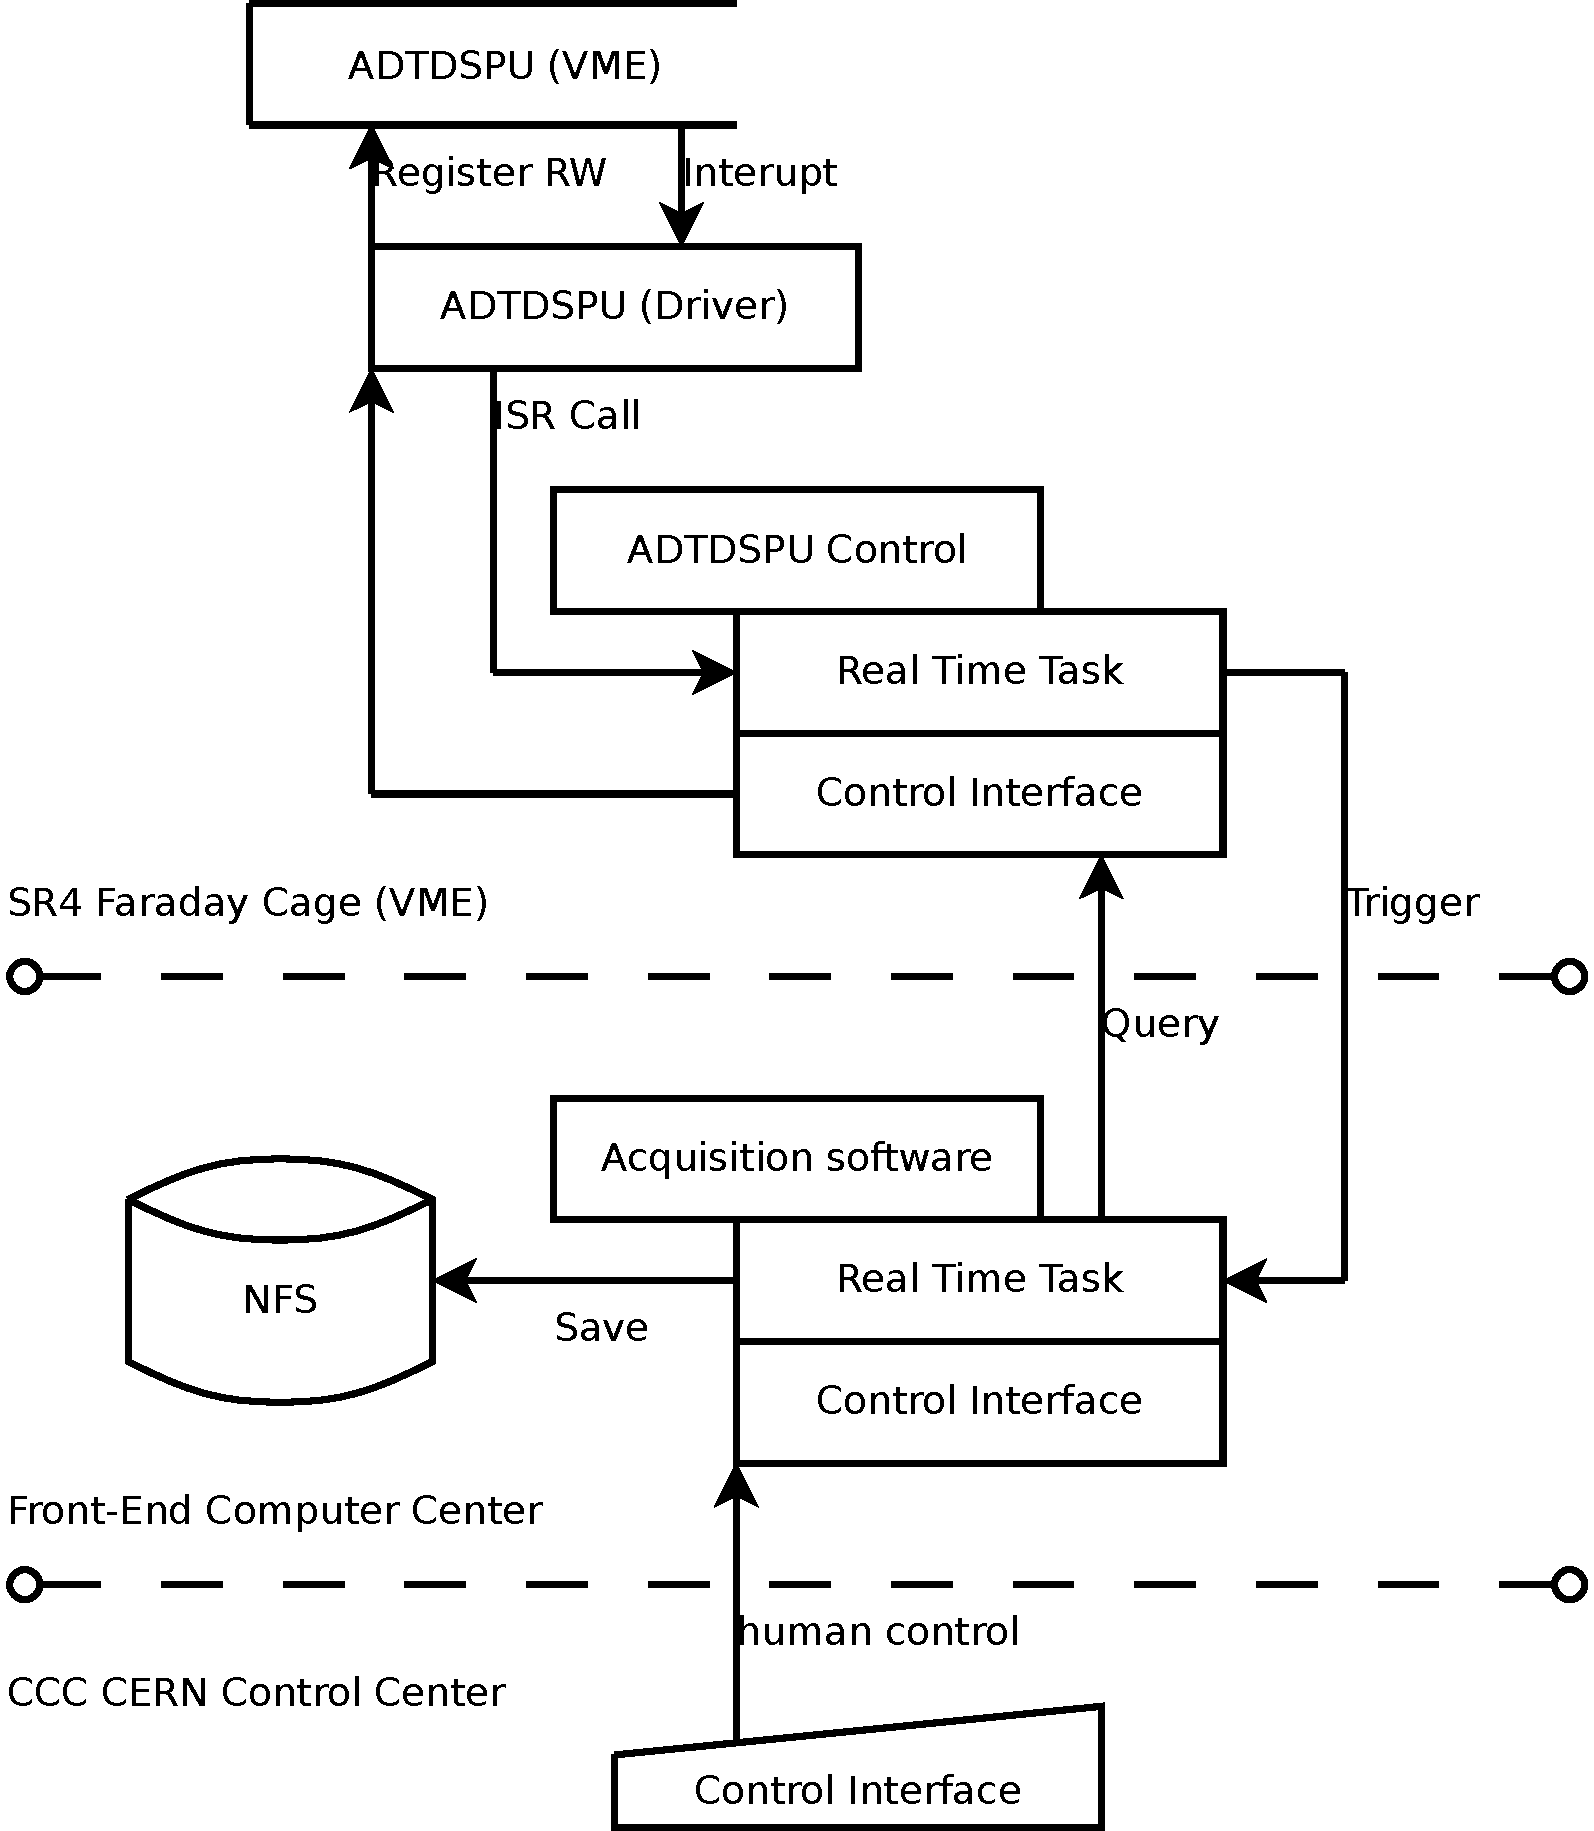
\includegraphics[scale=0.3]{ImplementedSoftFesa.pdf}
\end{figure}

In the final version the software will be merged in single executable that should run on the \gls{GPU}-enabled machine. This solution has been put into place because the present hardware is still in development and there is no way of acquiring the full 2880 bunches of the machine, the hardware is receiving the acquisition data but the \gls{VME} is not fast enough to transfer it to the \gls{CPU}.

	\subsection{ADTDSPU control software}

	The first layer that was needed is a driver that can control the \gls{VME} card and forward the interrupts. This is using standard driver framework from the \gls{CO} group at \gls{CERN}.

	Then the normal \gls{FESA} environment is used to develop a higher level software to control the card. This particular card need real time task to react to interrupt coming from the hardware to inform when new acquisition is ready to be read.

	\subsection{Acquisition software}

	The acquisition software was used to check that the idea of getting the tune out of the DSPU card was doable and being able to log the acquisition to file to be checked and processed separately.

	\begin{figure}[H]
	\caption{Tune acquisition software interface}
	\centering
	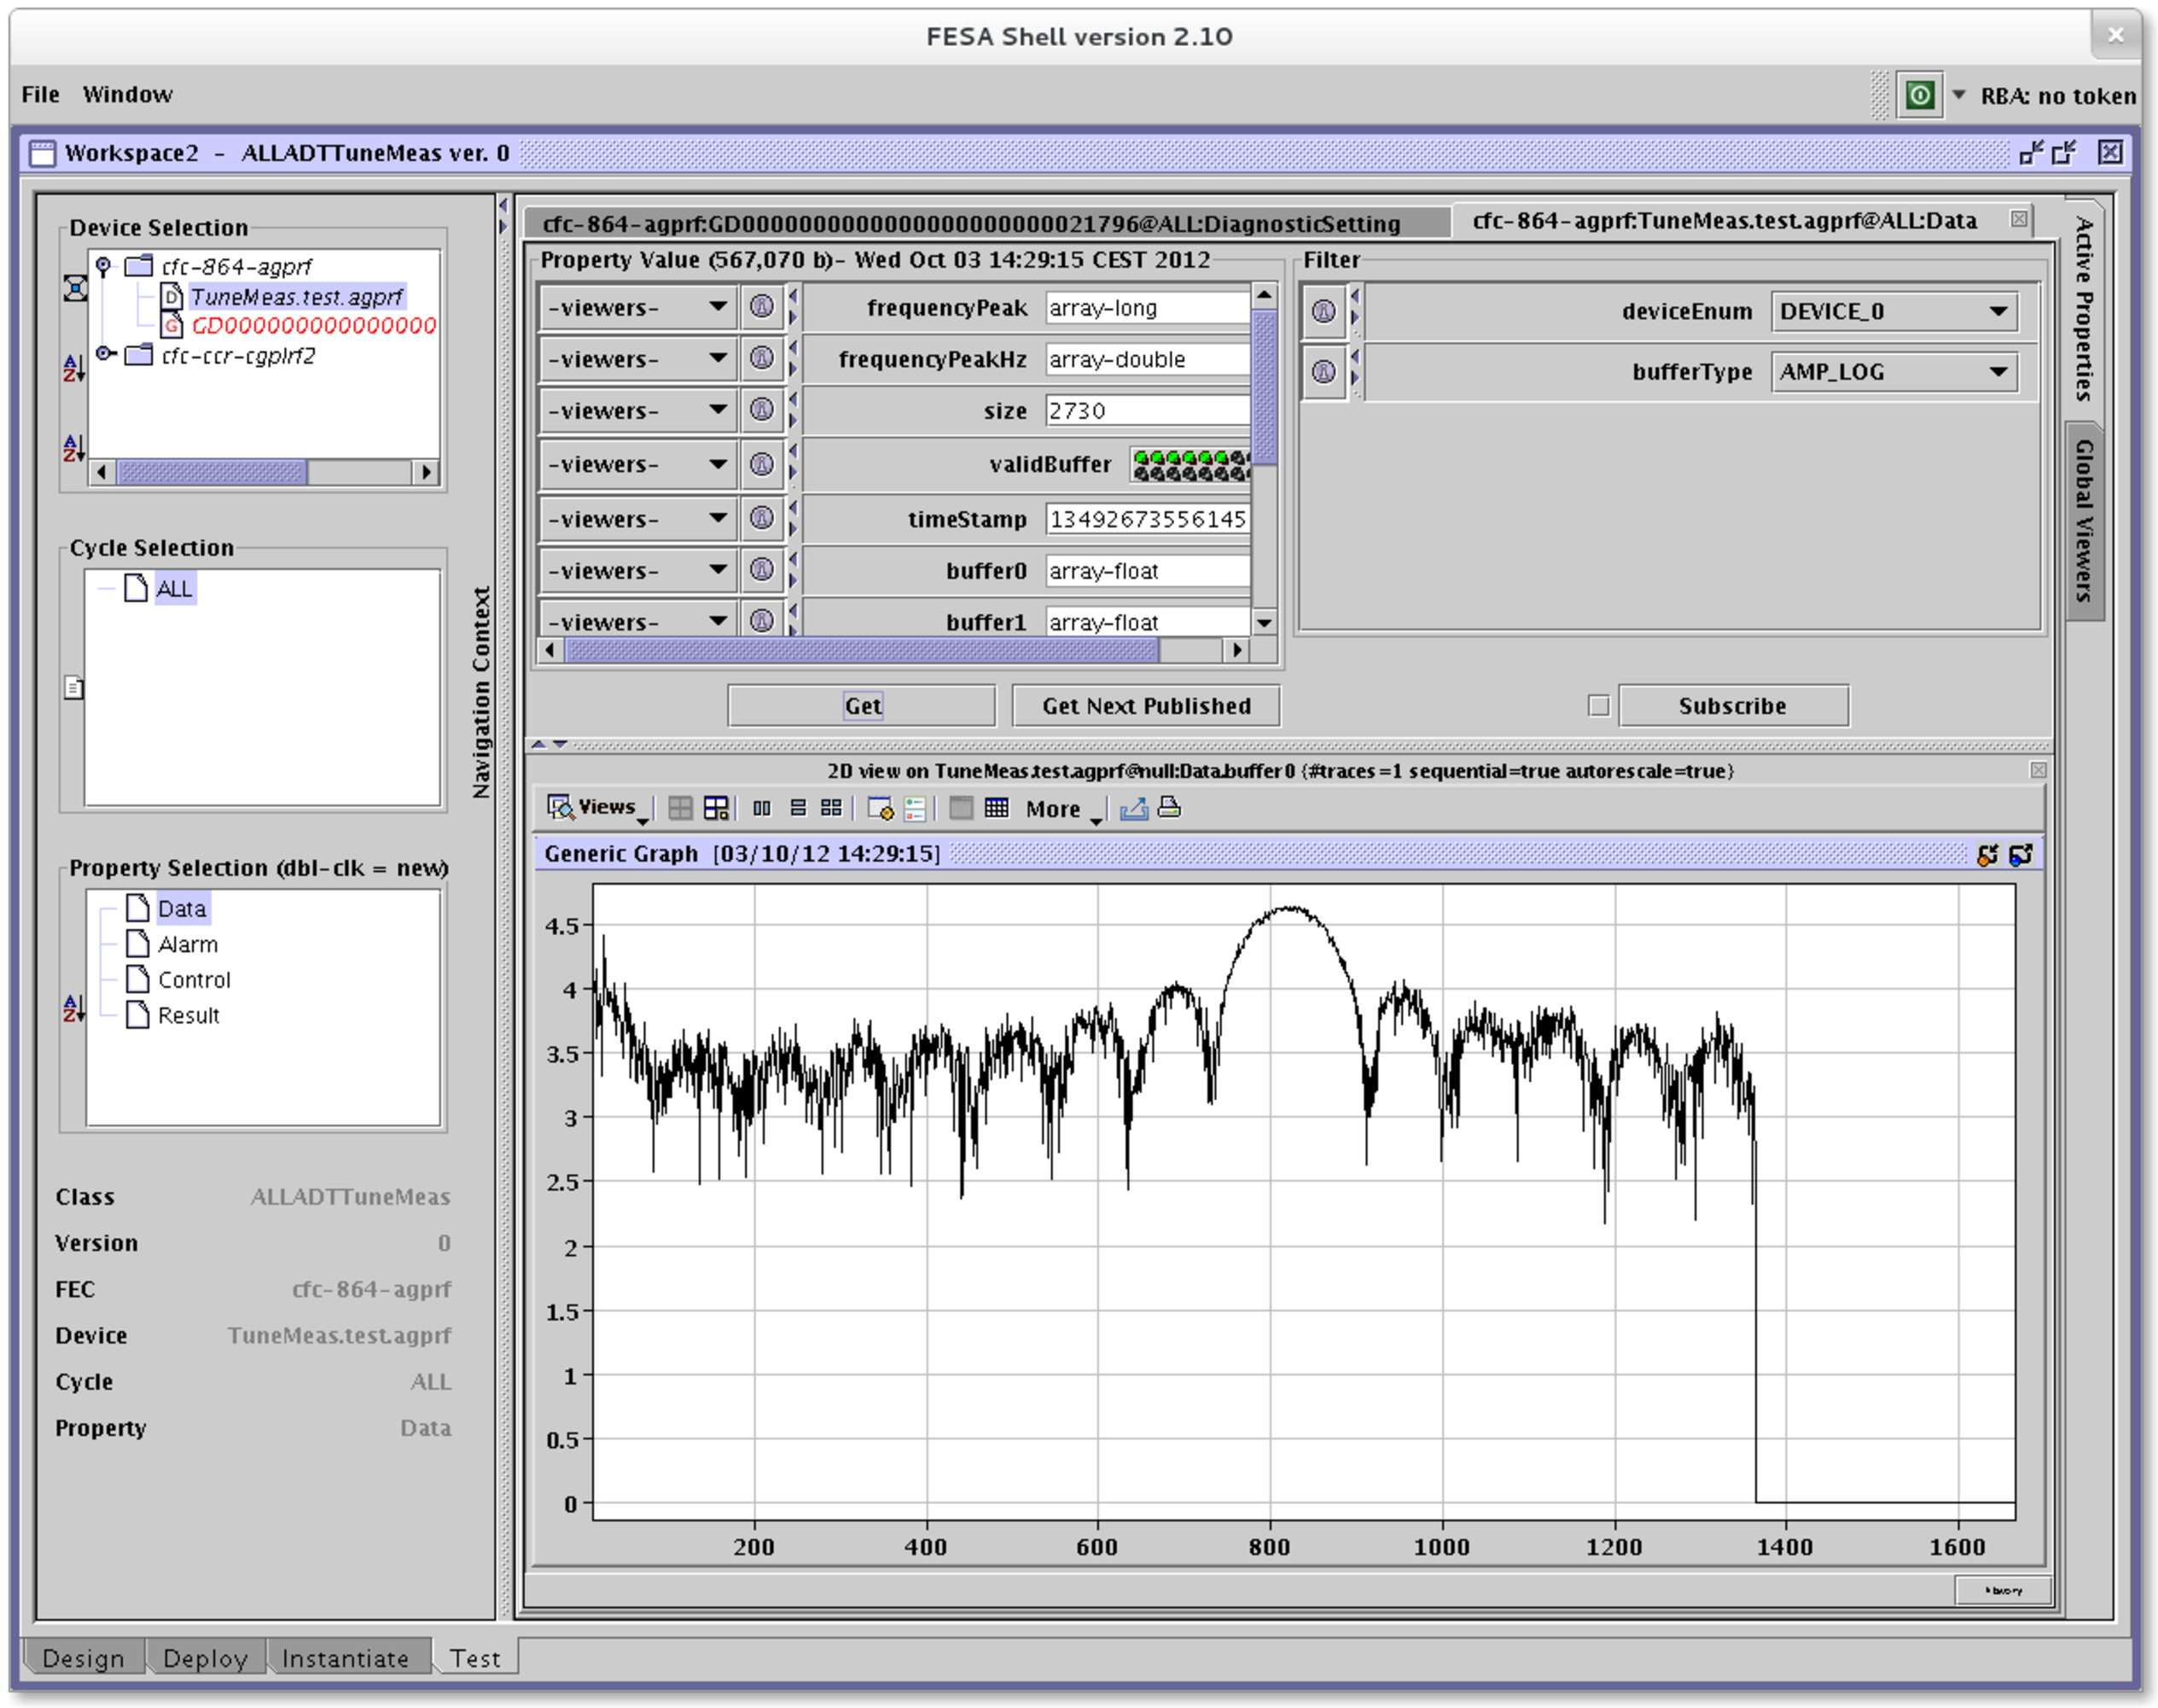
\includegraphics[scale=0.3]{amplitude_log.pdf}
	\label{fig:tuneacq}
	\end{figure}

	It uses \gls{CMW}, a library used at \gls{CERN} to communicate between different layers of the accelerators control software, to connect to the the ADTDPSU control software and get the data when they are published (at interrupt time).

	It is then able to compute the acquisition \gls{FFT} using \gls{FFTW} and display it to the operators in the \gls{CCC} where all the eight accelerators of \gls{CERN} are controlled. On the interface you can decide witch type of graph you want to see and also enable saving the data into files to be processed by the data analysis software.

	\subsection{Data analysis software}
	\label{sec:data_analysis_software}

	The data analysis software is a set of modules that can be enabled or bypassed to test the the usefulness of an algorithm. As we have precise time allocated to make the full computation this allow to test the different modules.

	\begin{figure}[H]
	\caption{Time flow with different implementations and with 3000 bunches of 
	2048 points each.}
	\centering
	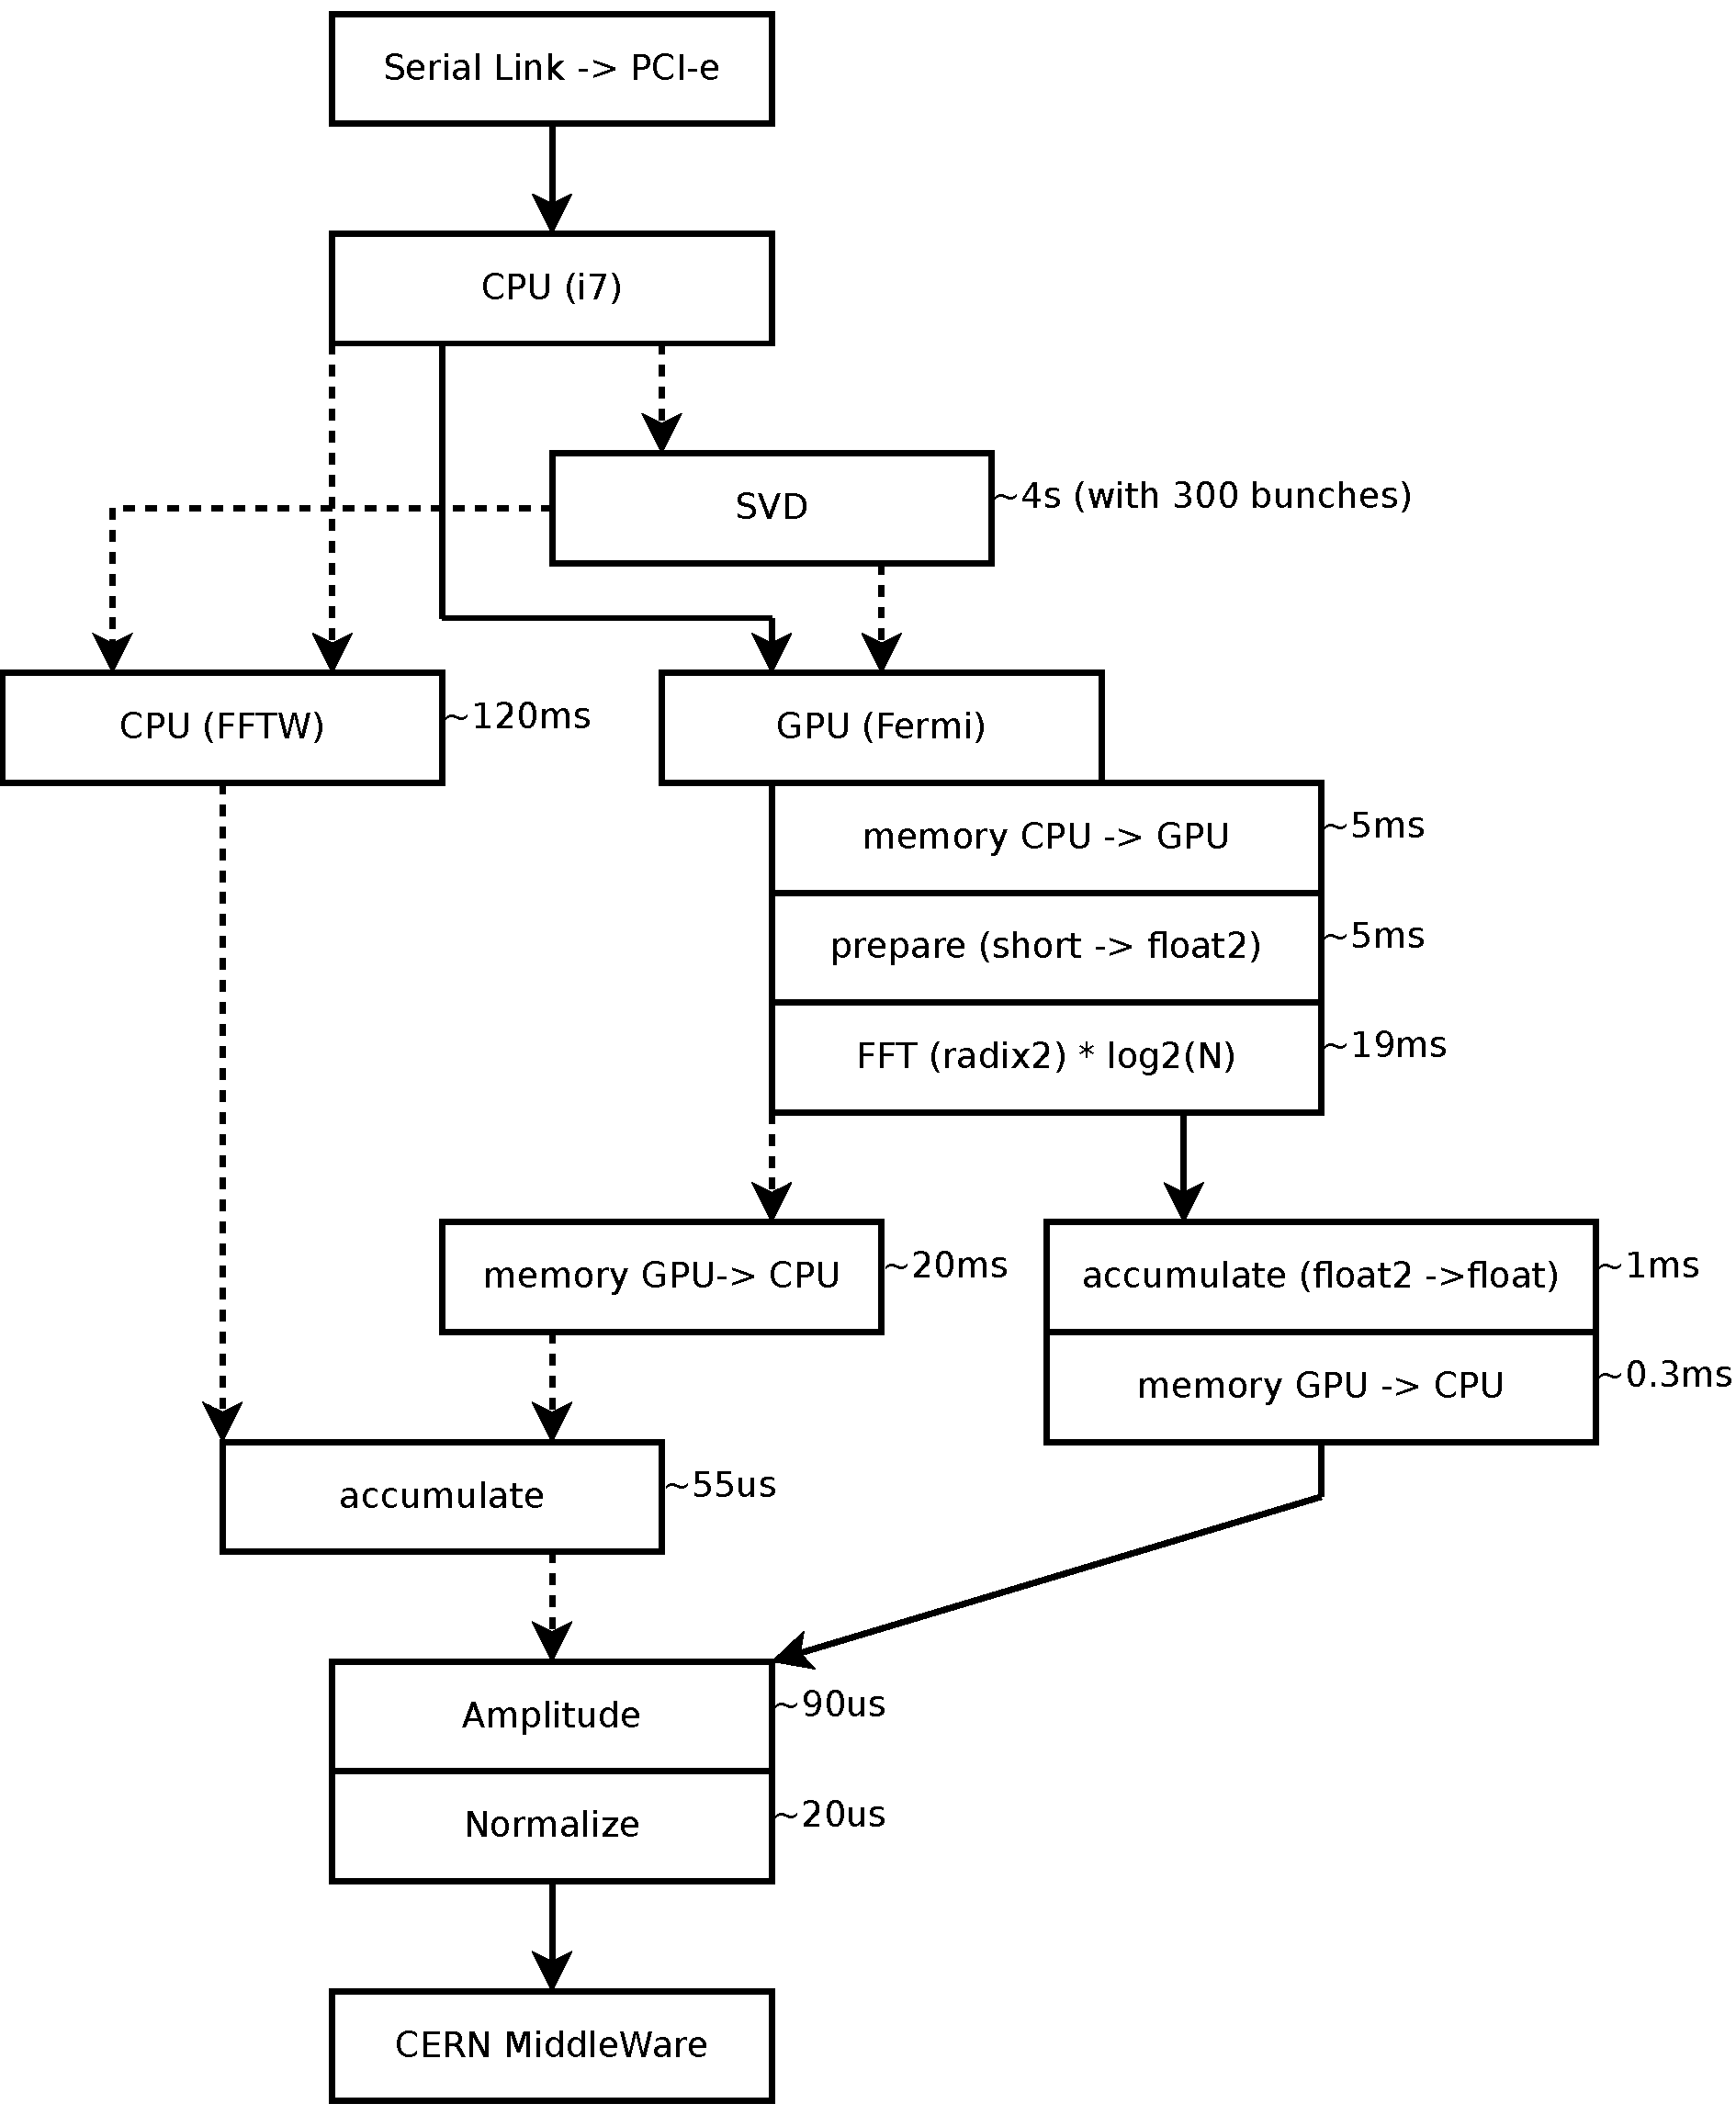
\includegraphics[scale=0.3]{PC-flow.pdf}
	\label{fig:PCFlow}
	\end{figure}

	The data is first loaded from the files that were written by the acquisition software. Then it is filtered by a notch filter as described in the notch section~\ref{sec:notch}. And finally to the different algorithms as shown in the figure~\ref{fig:PCFlow}.

	First optional step is \gls{SVD} this as described in Rama Calaga PHD thesis\cite{calaga06} and Wolfgang H{\"o}fle\cite{HofleChamonix12} should reduce noise in the signal result are seen in section\ref{sec:SVD}.

	Then come the the \gls{FFT} either using the \gls{GPU} or using the \gls{CPU}, actually you could use \gls{OpenCL} on the \gls{CPU} and test the whole \gls{OpenCL} path. The different path are due to memory copying, in the case of computation made on the \gls{GPU} you have to move the memory data from the \gls{CPU} central memory to the \gls{GPU} memory. this will described in section~\ref{sec:FFT}.

	To have a clear image and to combine the real and imaginary part of the \gls{FFT} we use the amplitude. It has been validated in the acquisition software as been the best metric, this could be changed as will in the final version. The amplitude is described in section~\ref{sec:amplitude}.

	As a final value is wanted we do the accumulation of all the bunches, it will give an average spectrum of the whole machine.

	The normalization step is just present for displaying the spectrogram (see section~\ref{sec:spectrogram}) and will not be needed for the final version.
 
\section{Notch filter}
\label{sec:notch}

A notch filter is used to cut the low frequencies, this doesn't change anything on the high frequencies, it won't be used in the final version. For every sample it takes the present sample and subtract the next element.

$$y_{[n]} = x_{[n]} - x_{[n + 1]}$$

This is a differential filter, as we are only interested into the higher frequency this has no incidence on our results and allow for a better visualization of the spectrograms.

\section{FFT}
\label{sec:FFT}

The Fourier transform is a mathematical operation that moves a function from a temporal domain to a frequency domain. In our case we are talking about \gls{DFT}, and in particular, the \gls{FFT}.

	\subsection{Definition}

	The \gls{DFT} is a discrete transform. It transform a function into another, which is called frequency domain, or simply \gls{DFT}, of the original function.

	$$ x_0,...,x_{N -1} \in \mathbb{C} $$

	$$ X_{k} = \displaystyle\sum\limits_{n = 0}^{N -1} x_{n}e^{-i 2 \pi k \frac{n}{N}} $$

	In order to compute the \gls{DFT} one must compute N number of values N times. The complexity is thus

	$$ \mathcal{O}(N^{2}) $$

	The most commonly used \gls{FFT} algorithms are based on a divide-and-conquer approach similar to the algorithm of Cooley and Turkey\cite{Cooley65}. The computation of a \gls{DFT} of length N is done by splitting the input sequence into a fixed small number of subsequences, compute their \gls{DFT}, and assemble the outputs to build the final sequence. If the split and assembly are linear in time the complexity becomes 

	$$ \mathcal{O}(N \log(N)) $$

   	\subsection{FFTW}

   	\Gls{FFTW} is an implementation of the \gls{DFT} that adapt to the hardware in order to maximize performance\cite{fftw05}. It is widely regarded as one of the fastest implementation of \gls{FFT} on \gls{CPU}.

   	It was selected as a reference for our the implementation, as \gls{OpenCL} can be run on directly on a \gls{CPU} is it possible to compare the time performances between the \gls{OpenCL} code running on \gls{CPU} and the \gls{FFTW} version see section\ref{sec:perf}.

   	It is under GPL license, can be purchased from the \gls{MIT} for commercial purposes and is used in many commercial and scientific package and software. As an example it is used in the MATLAB.

   	\subsection{FFT with OpenCL on GPU}

   	The \gls{FFT} version used in the software is derived from Eric Bainville's version. This is the reference implementation of \gls{FFT} on \gls{OpenCL} and is now the version distributed by Apple\cite{bainville11}. For the sake of simplicity we just used the radix2 version of the implementation but it is probably possible to gain even more time by using a higher radix.

   	On \gls{GPU} the \gls{OpenCL} result is the same than the one using \gls{FFTW} with the advantage to be faster on recent \gls{GPU}. The kernel is called a number of time equal to the size of the vector and then 11 times in the case of 2024 points ($\log{2^{11}} = 11$). A second dimension is used to pass the multiple vector.

   	\subsection{FFT with OpenCL on CPU}

   	As \gls{OpenCL} is also able to run on \gls{CPU} we used the same code than the one used on \gls{GPU} on \gls{CPU} and got the same results. It is interesting to note also that the time is very similar to the \gls{FFTW} version.

\section{Amplitude}
\label{sec:amplitude}

The amplitude is the length of the complex vector composing the \gls{FFT}, it is equal to the euclidean norm. 

$$ \mid x + i y \mid \equiv \sqrt{x^2 + y^2}$$ 

There is different ways to compute the norm of a 2-dimensional vector in \gls{OpenCL} and all of them seams to work equally on our test.

\section{SVD}
\label{sec:SVD}

It was suggested by Rama Calaga\cite{calaga06} to use \gls{SVD} in order to diminish the noise and improve the visibility of the tune in the frequency domain. The idea is to take the raw data and use the multiple bunch as a second dimension of our SVD then apply the algorithm and suppress the values in the $\Sigma$ matrix that are off a certain scale, finally recompose the M matrix and hopefully have less noise in it.

$$M = U \Sigma V^{T}$$ 

This was first tested on generated data by Wolfgang H{\"o}fle\cite{HofleEvian10} unfortunately we have only 6 bunches in our dataset per acquisition so it is not possible to make this work with the present set up. The $\Sigma$ matrix is only 6 by 6 values so it is not easy to suppress values in notable fashion.

Taking more than one acquisition can at least give some idea on the speed of processing. So SVD was implemented using the GNU Scientific Library (only double precision float for SVD). The problem is that correlation between beam of the same acquisition make the process a lot faster than uncorrelated bunches.

\begin{table}[H]
	\caption{SVD with vary heavily with correlation of bunches}
	\label{tab:SVD}
	\centering
	\begin{tabular}{|l|l|l|}
		\hline
			Bunches & Acquisitions & Time \\
		\hline
			5 & 20 & 0.15 s \\
			4 & 25 & 0.30 s \\
			2 & 50 & 2.04 s \\
			1 & 100 & 16.9 s \\
		\hline
	\end{tabular}
\end{table}

So it is very difficult to estimate the time the computing with the real data would take, but we have to keep in mind that these computation where done using double precision as single would probably be enough, these computation were only done using a single thread (SVD is quite difficult to parallelize) and only done on \gls{CPU}.

There is a way to make these computation on \gls{GPU}\cite{Lahabar09} and the estimation are around 5 times better than on \gls{CPU}. As soon as we have better data set (witch will require hardware upgrade) we can further investigate on this.

\section{Performances}
\label{sec:perf}

Computation were made by accumulation to simulate the number of bunches that could be present in the final version (2880). As 6 bunches were acquired we used 500 successive acquisition to make it close to the 2880 and have a safe margin.

Different strategy were used to try to improve performances as shown in figure\ref{fig:PCFlow}. But also use of pipelining (not used on the figure as it is difficult to estimate time when using pipelining) and test on different hardware.

The hardware used was mainly the Tesla M2090 based on a Fermi chip this chips has more cores than a CPU and we can see an improvement in respect of computing speed as shown on the table \ref{tab:speed}. The table \ref{tab:fermi} show the characteristic of the Tesla Fermi card family.

\begin{table}[H]
	\caption{NVIDIA Fermi hardware available on the market\cite{nvidia}}
	\label{tab:fermi}
	\centering
	\begin{tabular}{|l|l|l|}
		\hline
			Features & Tesla M2090 & Tesla M2075 \\
		\hline
		\hline
			Peak double performance & 665 Gflops  & 512 Gflops \\
		\hline
			Peak single performance & 1331 Gflops & 1030 Gflops \\
		\hline
			Memory bandwidth (ECC off) & 177 GB/sec & 150 GB/sec \\
		\hline
			Memory size (GDDR5) & 6 GB & 6 GB \\
		\hline
			CUDA cores & 512 & 448 \\
		\hline
	\end{tabular}
\end{table}

But if we have a look on the different card that are available today on the market we see that the new generation should have even better result and are available today. These card show around 5 times the number of \gls{CUDA} core and around 10 times the number of \gls{flops} as shown on table \ref{tab:kepler}.

\begin{table}[H]
	\centering
	\caption{NVIDIA Kepler hardware available on the market\cite{nvidia}}
	\label{tab:kepler}
	\begin{tabular}{|l|l|l|l|}
		\hline
			Features & Tesla K20X & Tesla K20 & Tesla K10 \\
		\hline
		\hline
			Peak double performance & 1.31 Tflops & 1.17 Tflops & 190 Gflops \\
		\hline
			Peak single performance & 3.95 Tflops & 3.52 Tflops & 4577 Gflops \\
		\hline
			Memory bandwidth (ECC off) & 250 GB/sec & 208 GB/sec & 320 GB/sec \\
		\hline
			Memory size (GDDR5) & 6 GB & 5 GB & 8GB \\
		\hline
			CUDA cores & 2688 & 2496 & 3072 \\
		\hline
	\end{tabular}
\end{table}


   \subsection{Pipelining}

   To improve the performances one of the options to try is to remove all waiting time between the different operations on the \gls{GPU}, as shown on the figure \ref{fig:PCFlow} the different operations done on the \gls{GPU} that are done sequentially could be pipelined.

   Pipelining mean that you won't wait for all the sub-operations to be finished before starting the next one. The first operation is copying the memory from the \gls{CPU} to the \gls{GPU} this takes a certain time but as soon as some of the data is copied the computing could start.

   In \gls{OpenCL} the different commands are queued and this command queue can be flushed. to make the pipelining work the only thing to do is to only flush at the end when all the computing has been queued.

   In our case this mean that the copying of the data from \gls{CPU} to \gls{GPU} the preparation of the data the \gls{FFT} itself the amplitude computation, the accumulation and getting back the values to the \gls{CPU} is queued together in one go.

   That allow us to have a 10\% improvement on performances, but it is difficult then to estimate the computing time of individual steps so the values shown on figure \ref{fig:PCFlow} are without pipelining.

   \subsection{Memory}

   Copying memory from and to the \gls{GPU} can be expansive time wise, as shown on figure \ref{fig:PCFlow} copying 3000 times 2024 values in short (2 bytes) take around 10 ms. This is the reason why it is important to make the accumulation on the \gls{GPU} because after the \gls{FFT} computation there is 3000 times 2024 complex values in float (8 bytes). It would have cost at least 40 ms to copy these values back to the \gls{CPU}. The 20 ms shown on figure \ref{fig:PCFlow} correspond to half the values because we can cut half of the result as the \gls{FFT} computed it in real only so the result is mirrored.
	
   \subsection{Time}

	\begin{table}[H]
		\caption{Speed for 3000 batch of 2048 points}
		\centering
		\label{tab:speed}
		\begin{tabular}{|l|lrrcr|}
			\hline
				Device & Type & Threads & Speed [GHz] & pipeline & Time [ms] \\
			\hline
			\hline
				Xeon X5650 & FFTW & 12 & 2.67 & N/A & 291 \\
				Xeon X5650 & OpenCL & 12 & 2.67 & enable & 284 \\
				Xeon X5650 & OpenCL & 12 & 2.67 & disable & 288 \\
			\hline
				i7-3720QM & FFTW & 8 & 2.6 & N/A & 310 \\
				i7-3720QM & OpenCL & 8 & 2.6 & enable & 272 \\
				i7-3720QM & OpenCL & 8 & 2.6 & disable & 273 \\
			\hline
			\hline
				Tesla M2090 & OpenCL & 512 & 1.3 & enable & 35 \\
				Tesla M2090 & OpenCL & 512 & 1.3 & disable & 37 \\
			\hline
				GeForce 650M & OpenCL & 384 & 0.9 & enable & 355 \\
				GeForce 650M & OpenCL & 384 & 0.9 & disable & 365 \\
			\hline
		\end{tabular}
	\end{table}

	Time performances were computed using the timing library from boost \cite{boost} on different hardware, \glspl{GPU} and \glspl{CPU}, with and without pipeline enable as shown on table \ref{tab:speed}.

	The time performances between \gls{FFTW} and \gls{OpenCL} on \gls{CPU} is very close, so the radix 2 implementation used must be good and we can hope the performances on \gls{GPU} could then be fairly compared with \gls{FFTW}.

	On a dedicated \gls{GPU} like the Tesla M2090  the performances are around 10 times better than on a modern \gls{CPU}. This is very encouraging and means that on last generation hardware we should be able to achieve even better performances.
	
\section{Spectrogram}
\label{sec:spectrogram}

A Spectrogram is a time-varying spectral representation of a signal. the signal is transformed via \gls{FFT} from time domain to spectral domain, each transformation makes a line in this case and is tagged with the time of the acquisition. the amplitude is used to have a single representation of both real and imaginary part of the result.

As we do a normalization by acquisition at the end of the computing we have a representation of the highest value with highest color (white) and if the amplitude is respectively weaker we have a darker representation of the color (black). To have a finer grain in representation intermediate color was chosen in this case blue as you can see in figure \ref{fig:squeeze} \ref{fig:ramp} and \ref{fig:adt_off}.

\begin{figure}[H]
	\caption{Spectrogram with ADT off on the 16 October 2012 on vertical beam 1 during squeeze and collision}
	\label{fig:squeeze}
	\centering
	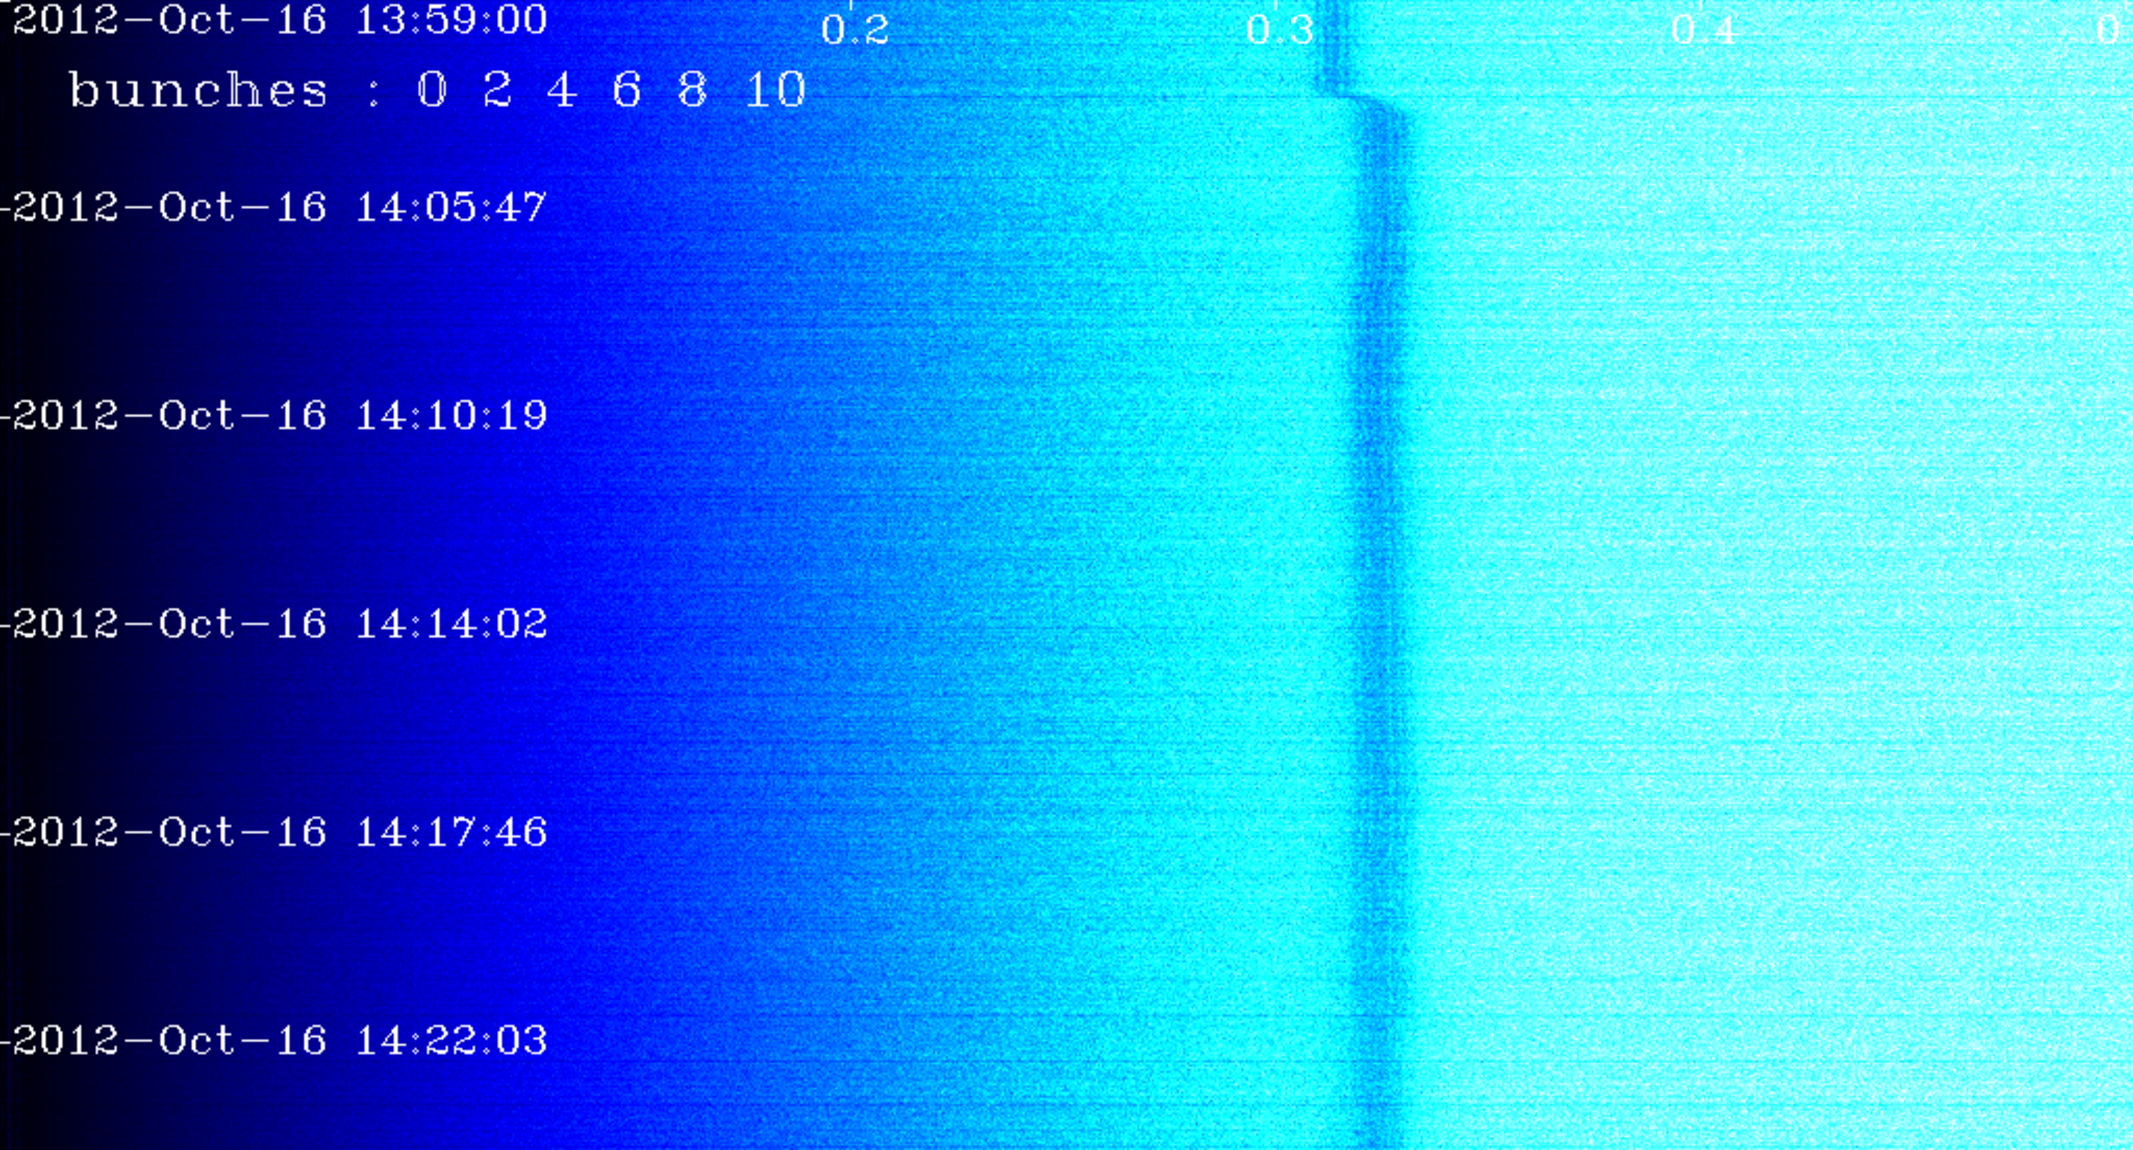
\includegraphics[scale=0.3]{md-121016-vb1-m1-6bunches-10acc-1359-1425-collision.pdf}
\end{figure}

The Spectrogram allow us to clearly see a mark in the signal that correspond to a region where the tune is suppose to be.